\documentclass{article}
\usepackage{graphicx}
\usepackage{float}
\usepackage{pdfpages}
\usepackage[legalpaper, portrait, margin=1in]{geometry}
\usepackage{enumitem}
\usepackage{minted}
\usepackage{amsmath}
\usepackage{cite}
\usepackage{hyperref}

\author{Xining Li, Debashis Kayal}
\title {Ensemble Learning Report}

\begin{document}
\maketitle

\section{Motivation}

Machine learning has already become ubiquitous in all aspects of modern-day living. Predictions from machine learning models are increasingly becoming an integral part of most computational systems around us. With the increased usage, achieving a higher prediction accuracy is an obvious need of the hour. 


In particular, existing machine learning algorithms are trying to find function within the hypothesis space that can approximate the following formulas.

\begin{equation}
    f^*(x) = {\mathrm {argmax}}_{Y=y} P (Y=y|X=x)
\end{equation}

The above formula does not address the existence of mislabeled data. Therefore, any classier's performance will be harmed by noise in dataset labels, which is to be anticipated; the relevant question is by how much?

Since machine learning’s prediction is directly dependent on the dataset that the models are trained upon, it follows that a high quality - properly labeled, de-duped, correct data is required. 

However in real life high quality data is hard to obtain - with the ever increasing “noises” which may cause data error. Typical data faults include: 

\begin{itemize}
    \item Repetitions (duplication)
    \item Mislabelings (label noise)
    \item Distortions ( intentional or unintentional deviation of data from its true or most accurate representation of the full picture)
\end{itemize}

\section{Label noise in ML}

Dataset noise can be either feature noise or label noise. Considering the relatively very high impact of label noise, we will focus on understanding its impacts.

Some research \cite{rolnick_veit_belongie_shavit_2018} has shown that ML systems can generalize and behave well even when trained with massive mislabeled data, but under certain specific circumstances:

\begin{itemize}
    \item The ML system must have a large enough parameter set to manage the complexity of the image classification task.  
    \item The training dataset must be very large – large enough to include many properly labeled examples, even if most of the training data is mislabeled. With enough good training samples, the ML system can learn accurate classification by finding the ‘signal’ buried in the label noise.
    \item The mislabeling is random and does not form a pattern of its own
\end{itemize}

However most ML models face challenges that make label noise a sufficiently big problem. These pose  complications such as:

\begin{itemize}
    \item Unavailability of large training datasets
    \item Systematic, pattern-building labeling errors that confuse machine learning.
\end{itemize}

The performance of any classifier, or for that matter any machine learning task, depends crucially on the quality of the available data.


Aim of this paper is to explore the usage of ensemble methods in machine learning and how it can help increase the fault-tolerancy of the models.

It has already been established that Ensemble Machine Learning improves accuracy by reducing the variance compared to using a single model. Additionally, ensemble techniques also improve the average performance of a model thus contributing to the robustness of the model. Some ensemble methods like boosting (XGb) are robust enough to take care of missing data on their own.

\section{Ensemble Learning in ML}

The premise of using ensemble-based decision systems in our daily lives is fundamentally not different from their use in computational intelligence. We consult with others before making a decision often because of the variability in the past record and accuracy of any of the individual decision-makers \cite{martin_2018}.

Ensemble method is the machine learning technique that involves combining several base models to create a better predictive model. Idea is that accuracy of the ensemble model is much better than the individual learner models. By using ensemble methods we aim to gain:


\begin{itemize}
    \item Higher predictive accuracy (lower errors)
    \item More consistency (by avoiding overfitting)
    \item Reduce bias and variance errors
\end{itemize}

\section{Different Popular Techniques of Ensemble Learning}

\begin{figure}[H]
    \centering
    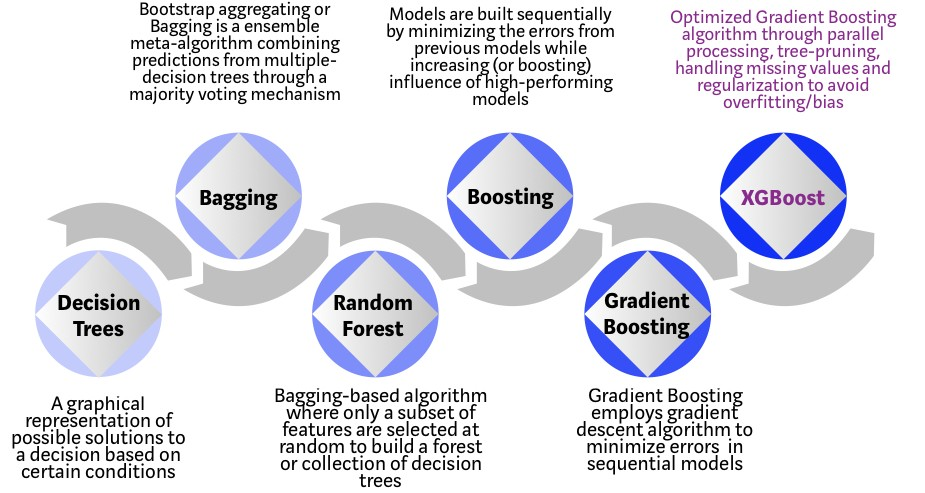
\includegraphics[width=8cm]{report-imgs/img1.jpeg}
    \caption{Different Popular Techniques of Ensemble Learning}
    \label{DifferentPopularTechniquesOfEnsembleLearning}
\end{figure}

The \autoref{DifferentPopularTechniquesOfEnsembleLearning} shows different popular techniques of ensemble learning. 

\subsection{Bagging: Bootstrap Aggregating}

Using the same learning models trained with different slices (subsets) of data randomly sliced from the whole training dataset and then voting (majority) to arrive at the output.


\begin{enumerate}
    \item Random splitting of the training data set into multiple samples. 
    There may be some data overlap between samples (since data slicing is random).
    \item Base model selected is trained using the bootstrap samples
    The selection of samples is also random thus the same sample may be used to train more than one model.
    \item Aggregating - the output from the different base models is used to arrive at the final output.
\end{enumerate}

For classification problems, a voting mechanism (usually majority vote) is used. 

For regression problems, the average of the output from the individual models is taken to arrive at the ensemble system output.

Both averaging and voting can be simple or weighted if relevant weights are available for use. 



\begin{figure}[H]
    \centering
    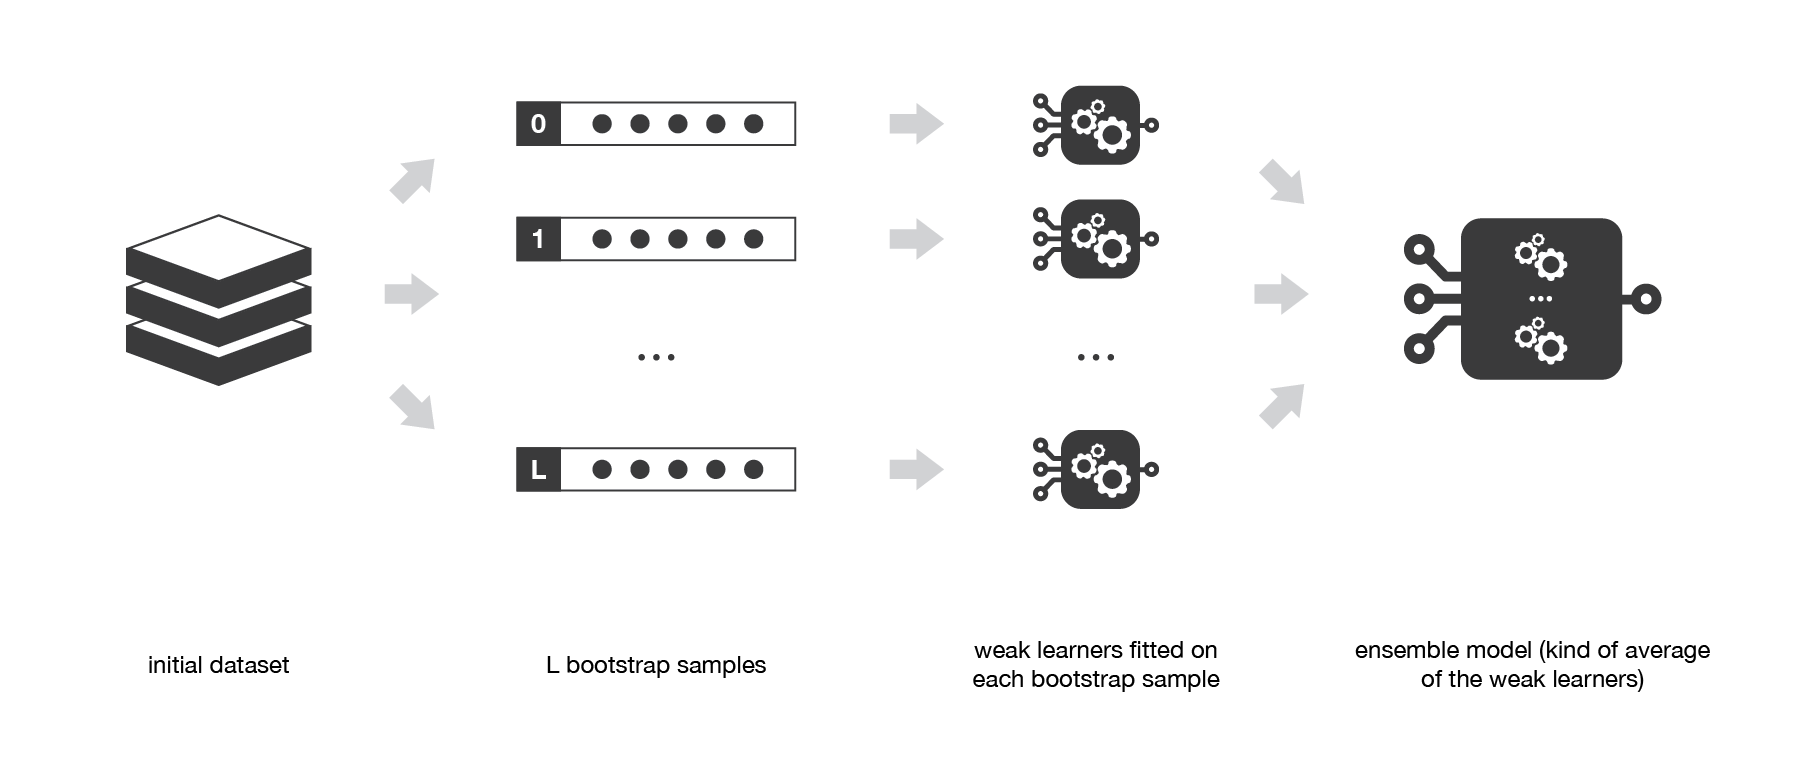
\includegraphics[width=8cm]{report-imgs/bagging.png}
    \caption{Bagging}
    \label{bagging}
\end{figure}

In Bagging, base models can train in parallel \cite{rocca_2021}. Bagging method is aimed at reducing variance. Since individual models can train in parallel - bagging is a parallel method of ensemble techniques.


Random Forests is a bagging method where deep trees are trained on bootstrap samples and combined to produce output with lower variance.In addition to the dataset sampling, it does sampling over features and uses a random subset of those features to build the tree. This ensures that not all decision trees take in the exact same training data. This sampling over features makes the process more robust to missing data as the trees take into account only features where data are not missing.

\begin{figure}[H]
    \centering
    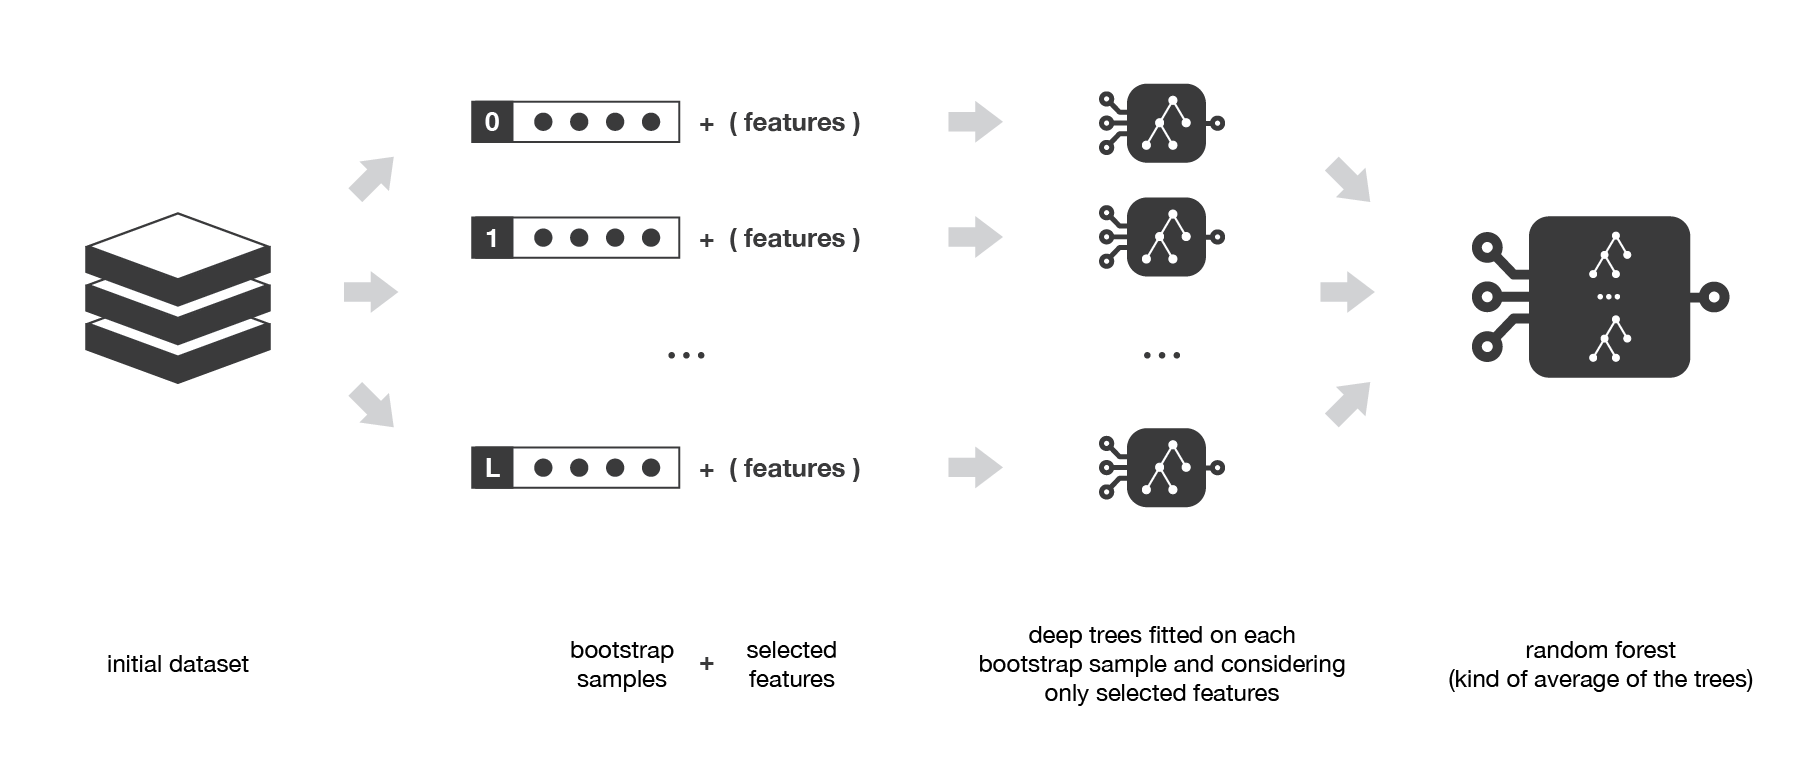
\includegraphics[width=8cm]{report-imgs/random-forest.png}
    \caption{Random forest is a bagging method that combines bagging with random feature subset selection}
    \label{randomForest}
\end{figure}



\subsection{Boosting}


Similar to bagging uses several base models but in a sequential iterative manner. Each sequentially fitted base learner focuses on improving the error output from the previous model. Thus we get a method that has lower bias and reduced variance.
Boosting is mainly focused at reducing bias. Two types of boosting techniques - Adaptive Boosting (ada boost) and Gradient boosting.
In Adaboost - the weight attached to each observation is changed while in Gradient Boosting the actual observation values are changed

\begin{figure}[H]
    \centering
    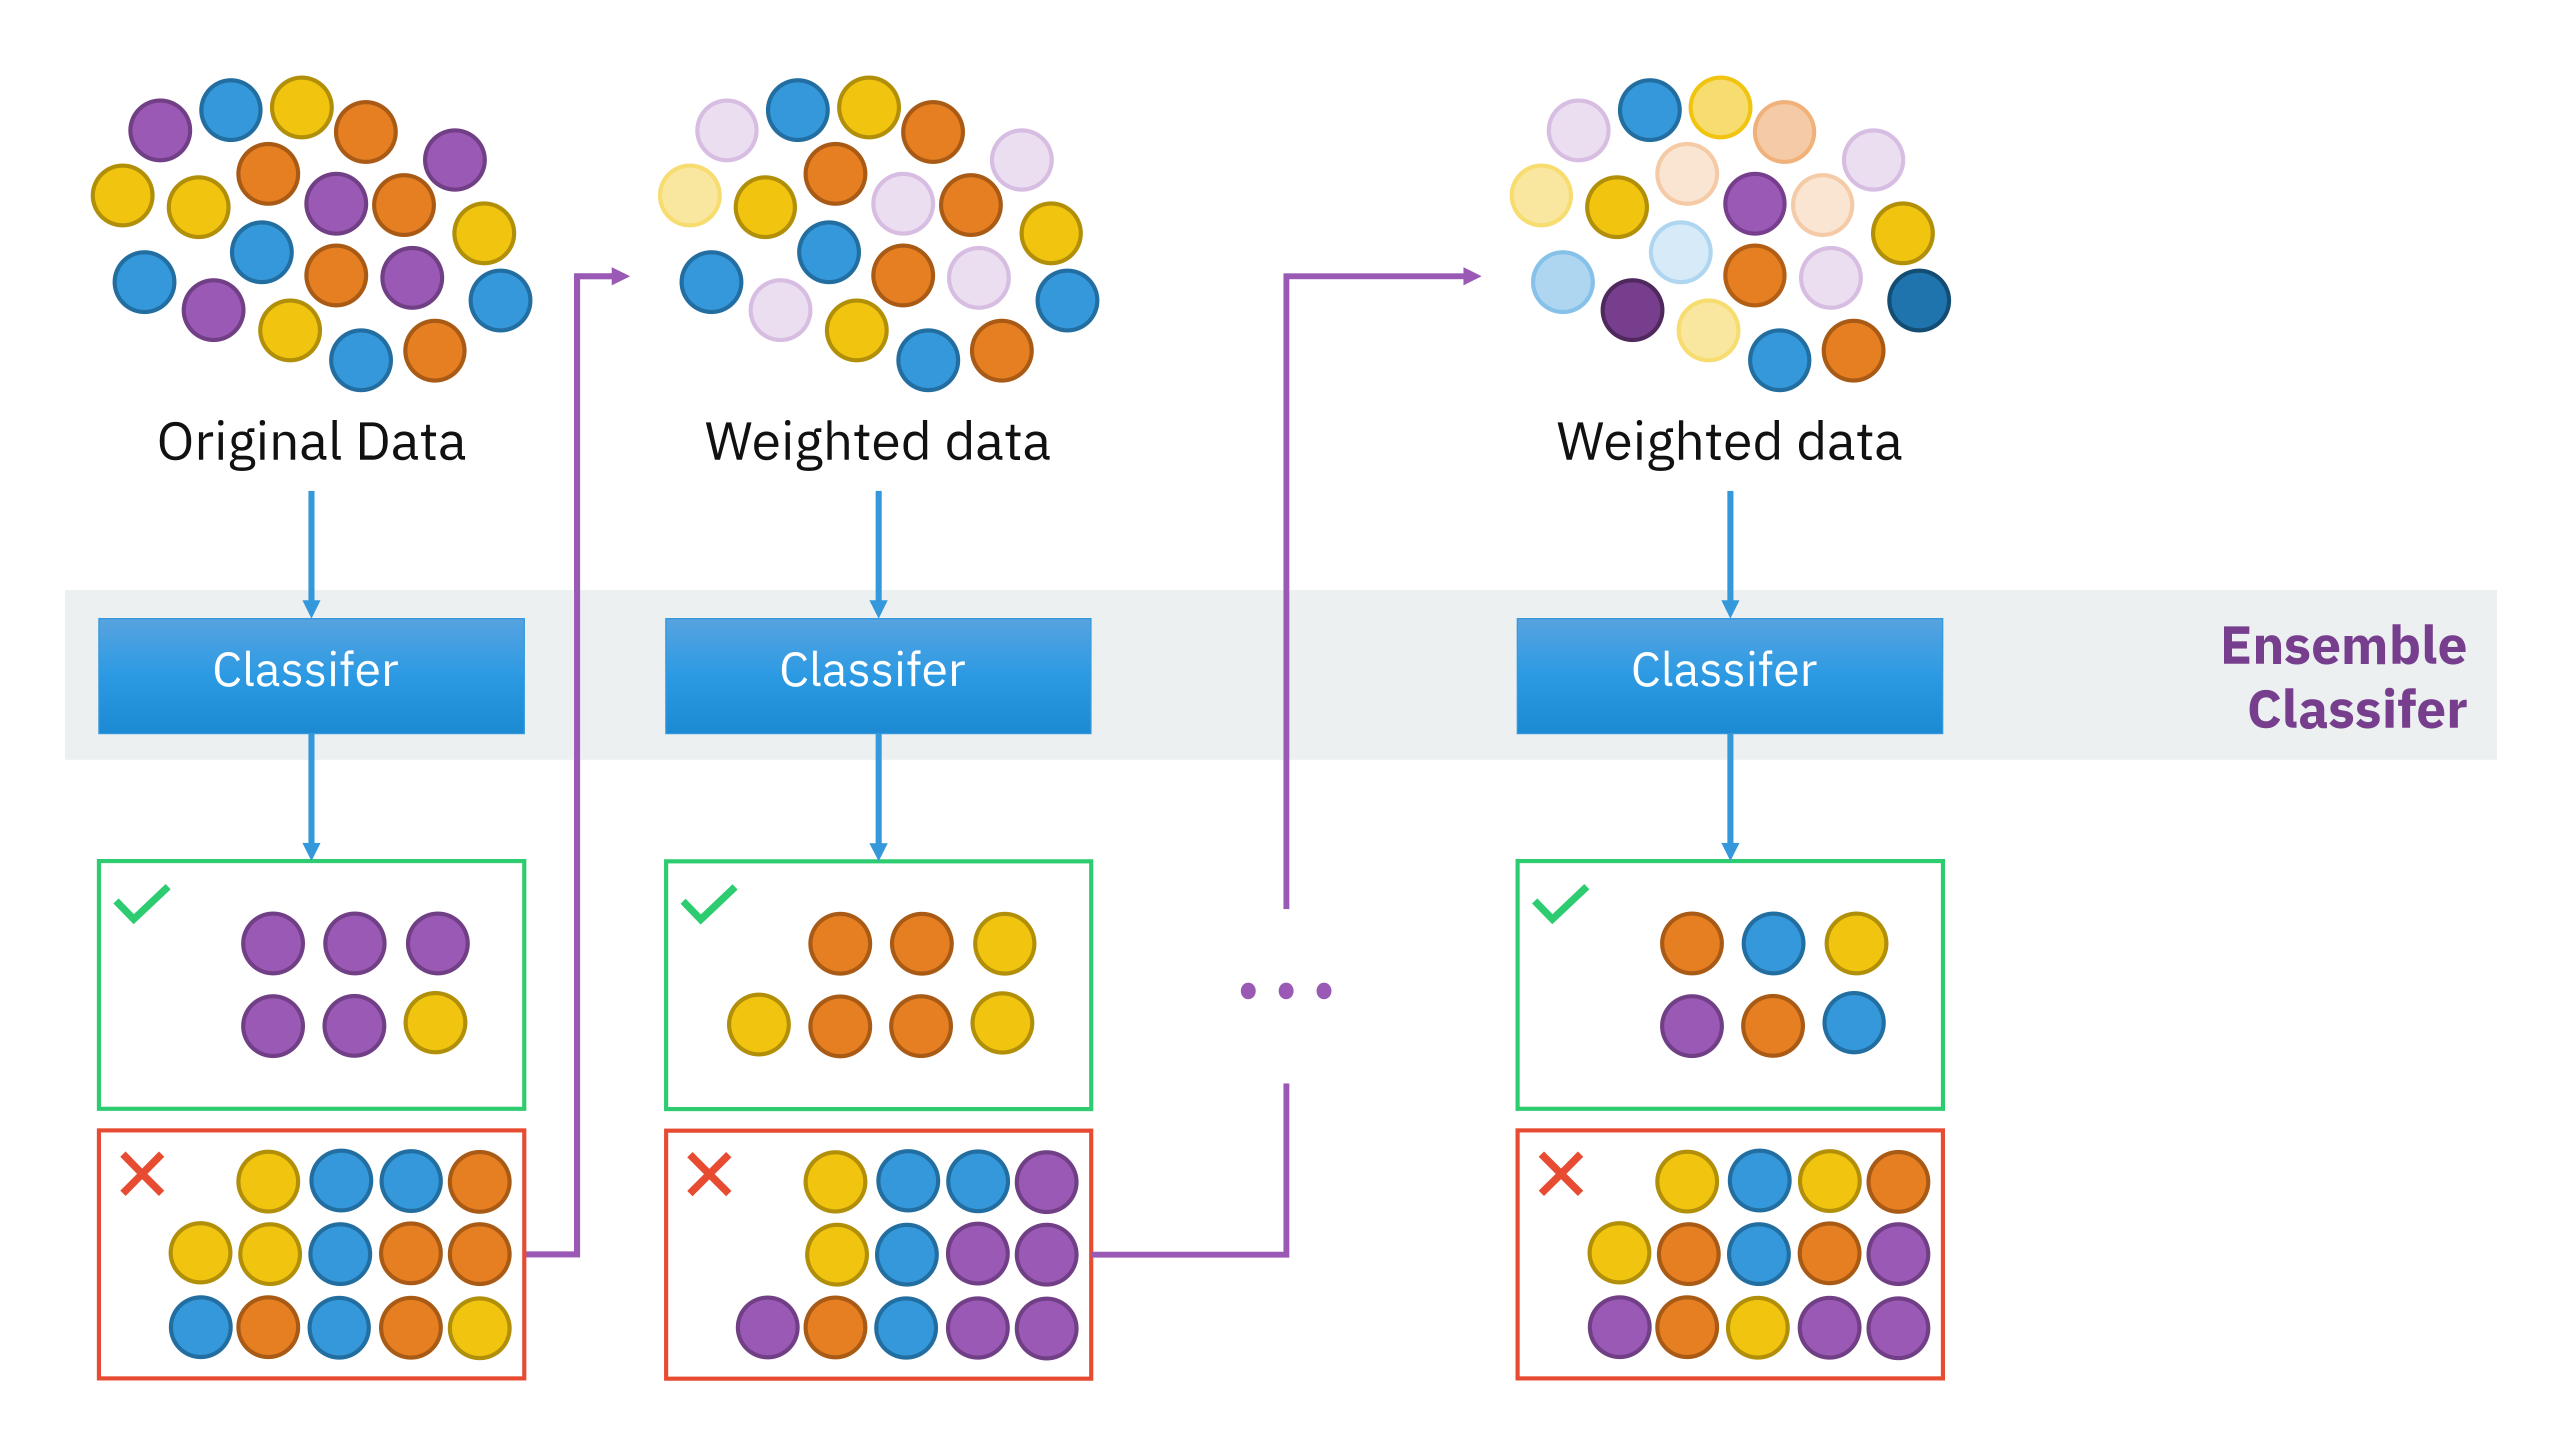
\includegraphics[width=8cm]{report-imgs/adaboost.png}
    \caption{Adaptive Boosting or Adaboost}
    \label{adaboost}
\end{figure}

Gradient boosting does not modify the sample distribution as weak learners train on the remaining residual errors  (i.e, pseudo-residuals) of a previous learner. By training on the residuals of the model, is an alternative means to give more importance to misclassified observations.


\begin{figure}[H]
    \centering
    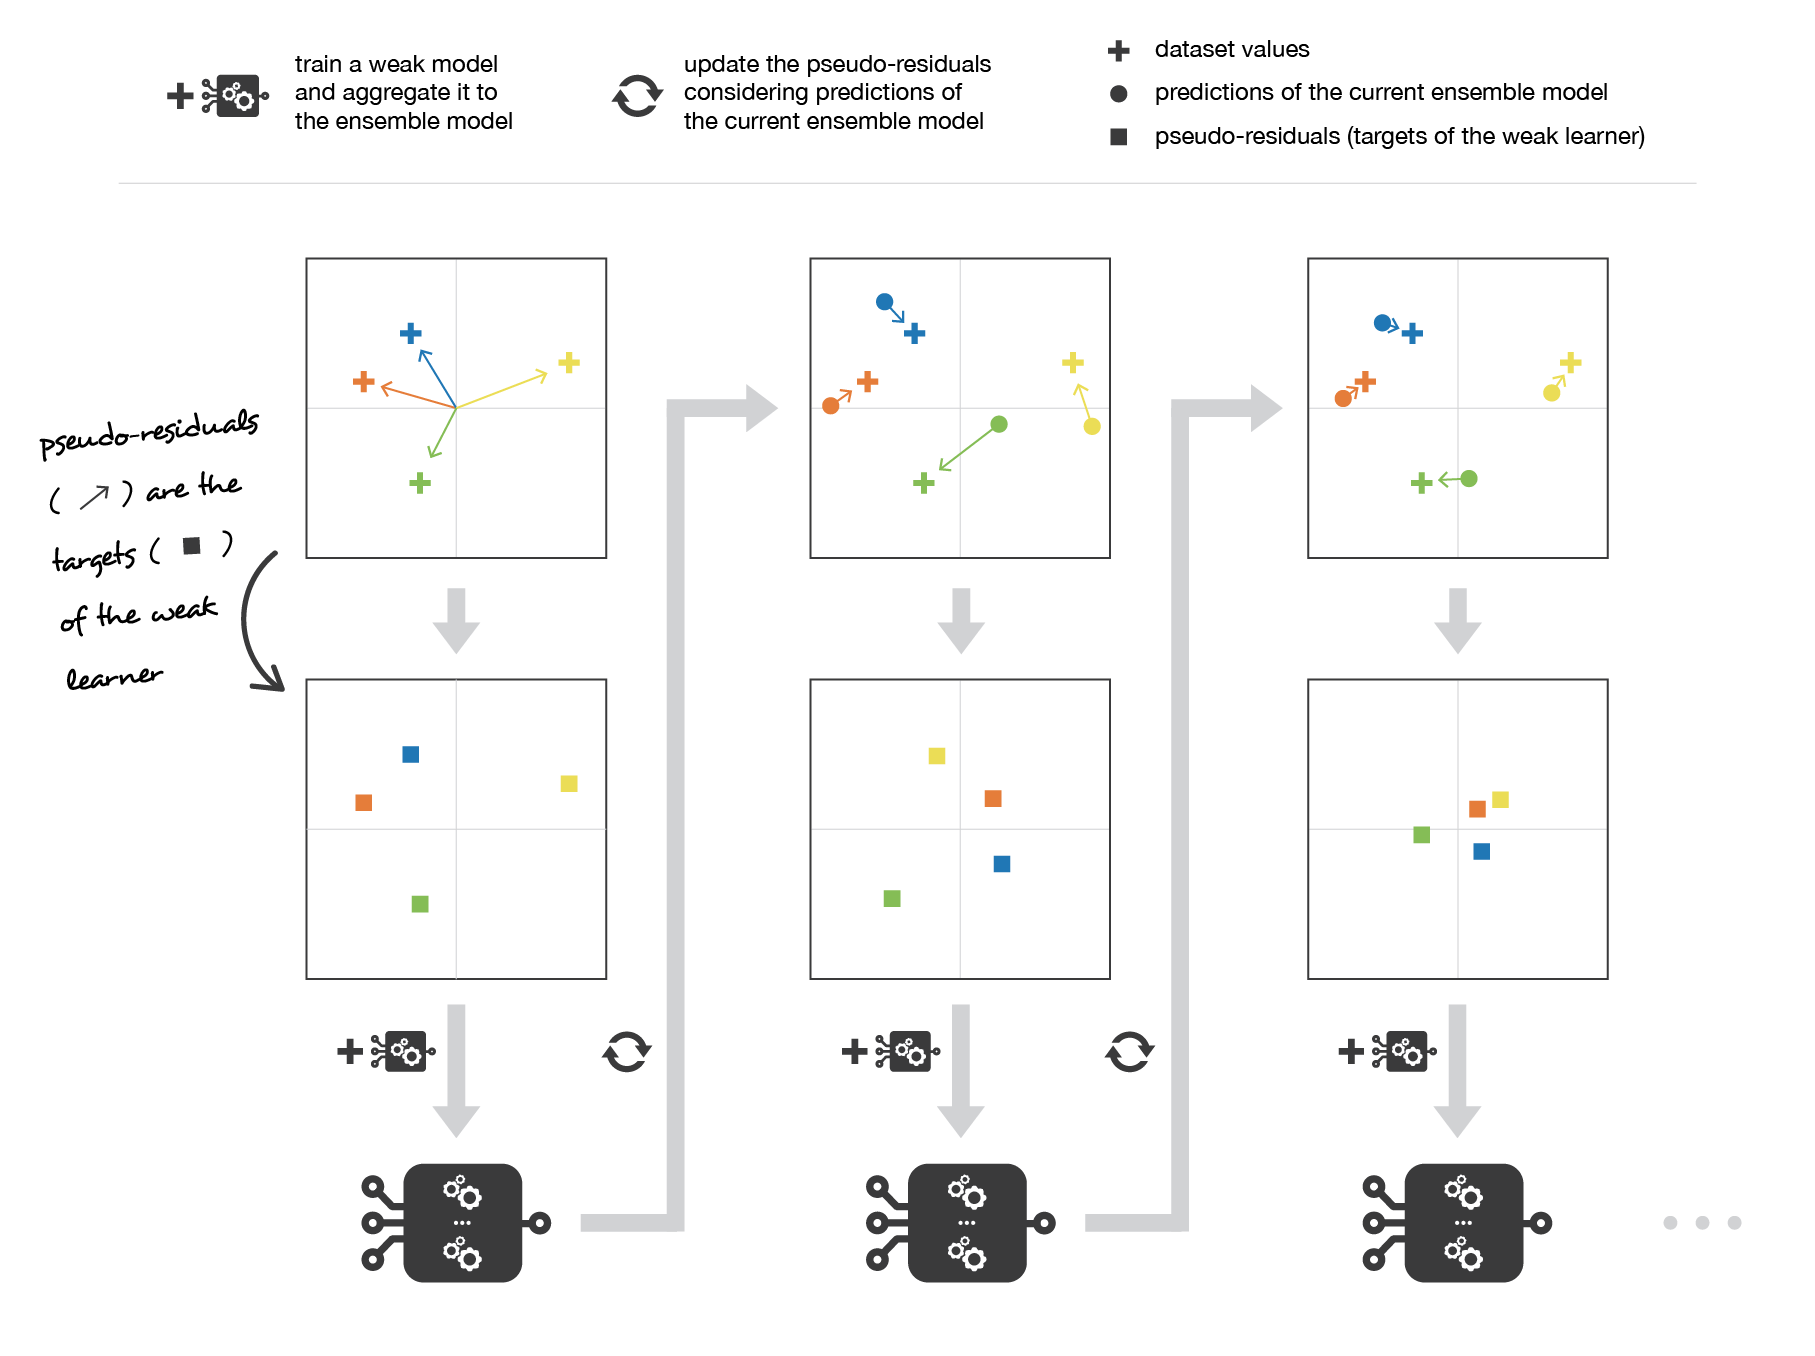
\includegraphics[width=8cm]{report-imgs/gradientboost.png}
    \caption{Gradient boosting}
    \label{gradientboost}
\end{figure}



Xtreme gradient boosting or XGB is a decision-tree-based ensemble Machine Learning algorithm that uses a gradient boosting framework. XGBoost is basically designed to enhance the performance and speed of a Machine Learning model. In prediction problems involving unstructured data (images, text, etc.), artificial neural networks tend to outperform all other algorithms or frameworks \cite{mujtaba_2021}. Like gradient boosting XGBoost also handles missing values in the dataset.  


\begin{figure}[H]
    \centering
    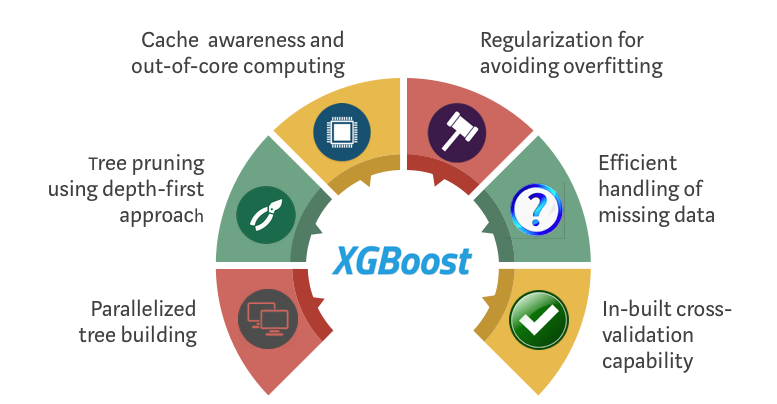
\includegraphics[width=8cm]{report-imgs/xgb.png}
    \caption{XGB steps}
    \label{xgb}
\end{figure}

\section{Objectives of this Paper}

In this project, we will be investigating the performance of ensemble learning algorithms with mislabeled data. We will be exploring dierent datasets, dierent machine learning algorithms, and dierent machine learning approaches; we will be juxtaposing training data without mislabeling and with mislabeling under the combinations of these.  
For the scope of this paper we have identified two major field of applications of ML: image recognition and natural language processing (NLP). 
Dataset Sourcing:
We will be sourcing our datasets from publicly available standard datasets (MNIST, CIFAR10…) for Image Recognition.


\section{Experiment}

\subsection{MINST Dataset}

The MNIST database of handwritten digits, available from this page, has a training set of 60,000 examples, and a test set of 10,000 examples. 

\inputminted[firstline=16,lastline=20,frame=single,framesep=10pt,fontsize=\footnotesize]{python}{minst/main.py}

\begin{figure}[H]
    \centering
    \includegraphics[width=\textwidth/2]{report-resources/minst/simple-minst-sample-1.pdf}
    \caption{MINST data handwriting example}
    \label{fig:let1}
\end{figure}

The Figure \ref{fig:let1} is a letter 1 in the MINST dataset. 

\subsubsection{Without Data Mislabeling}

The following algorithms run on the data without mislabeling. 

\inputminted[firstline=30,lastline=77,frame=single,framesep=10pt,fontsize=\footnotesize]{python}{minst/main.py}

\begin{figure}[H]
    \centering
    \input{report-resources/minst/f1_scores.tex}
    \caption{F1 Scores Table}
\end{figure}


\subsubsection{With Data Mislabeling}

We use the following data to intentionally create misslabeled data

\inputminted[frame=single,framesep=10pt,fontsize=\footnotesize]{python}{minst/do_miss_label.py}


\inputminted[firstline=93,lastline=142,frame=single,framesep=10pt,fontsize=\footnotesize]{python}{minst/main.py}


\begin{figure}[H]
    \centering
    \input{report-resources/minst/misslabeled_f1_scores.tex}
    \caption{Misslabled data F1 Scores Table}
\end{figure}

\subsection{The CIFAR-10 dataset}
The CIFAR-10 dataset consists of 60000 32x32 colour images in 10 classes, with 6000 images per class. There are 50000 training images and 10000 test images.

The dataset is divided into five training batches and one test batch, each with 10000 images. The test batch contains exactly 1000 randomly-selected images from each class. The training batches contain the remaining images in random order, but some training batches may contain more images from one class than another. Between them, the training batches contain exactly 5000 images from each class.

Here are the classes in the dataset, as well as 10 random images from each:

\begin{figure}[H]
    \centering
    \includegraphics[width=\textwidth/2]{report-resources/cifar-10-images/show_labels.png}
    \caption{CFAR10 data example}
\end{figure}

CFAR10 is a more complicated dataset, and we will be using the CNN for the feature extraction. 

After the feature extraction, we will be using the following ways for the classification. 
\begin{itemize}
    \item Softmax
    \item Random Forest
\end{itemize}

\subsubsection{Without Data Mislabeling}

\inputminted[frame=single,framesep=10pt,fontsize=\footnotesize]{python}{cifar10/main.py}

\begin{table}[H]
    \centering
    \begin{tabular}{rrrrr}
        CNN &  CNN+RandomForest   \\
        0.7885768705224767 &       0.8059692064910149  \\
    \end{tabular}
\end{table}

\subsubsection{With Data Mislabeling}

We applied 30\% of mislabeled data. 

\inputminted[firstline=32,lastline=54,frame=single,framesep=10pt,fontsize=\footnotesize]{python}{cifar10-mislabeled/main.py}


\begin{table}[H]
    \centering
    \begin{tabular}{rrrrr}
        CNN &  CNN+RandomForest   \\
        0.7371853465743461 &       0.7546625150853542  \\
    \end{tabular}
\end{table}
\bibliographystyle{IEEEtran}
\bibliography{report}

\end{document}


